\documentclass{article} % For LaTeX2e
\usepackage{nips14submit_e,times}
\usepackage{hyperref}
\usepackage{url}
\usepackage{graphicx}
\usepackage{amsmath}
\usepackage{amssymb}
\usepackage{anyfontsize}
\usepackage{subcaption}
\usepackage{titling}
\usepackage{array}
\usepackage{authblk}

\title{\vspace{-1.5cm} Unsupervised learning of probabilistic programs with latent predicate networks}

\author{Eyal Dechter,  Joshua Rule,  Joshua B. Tenenbaum\thanks{{\tt \{edechter, rule, jbt\} @mit.edu}}}
\affil{{\normalsize Department of Brain and Cognitive Sciences, MIT}}
\date{}

\newcommand{\fix}{\marginpar{FIX}}
\newcommand{\new}{\marginpar{NEW}}

\nipsfinalcopy % Uncomment for camera-ready version

\begin{document}
\maketitle

\vspace{-1cm}
\begin{abstract}

  Probabilistic programs successfully capture many aspects of the
  complex symbolic and statistical knowledge that human beings
  possess. Children are not born with this knowledge and must learn
  it, often in an unsupervised fashion. How can we flexibly and
  tractably learn probabilistic programs? We present early work on
  learning probabilistic programs with latent predicate networks
  (LPNs), a framework for unsupervised learning in a restricted space
  of probabilistic context-sensitive grammars. Specifically, we encode
  LPNs in the probabilistic logic programming language PRISM and use
  stochastic variational EM to infer its parameters. Using a small
  fragment of English sentences about number, we show that LPNs can
  recover much of the relevant conceptual structure necessary to
  complete novel sentences in this domain with high probability.

\end{abstract}

\section{Introduction}

%% Introduction idea
%% *** Probabilistic programs have been great models of human cognition
%% **** one-shot learning
%% **** linguistic pragmatics
%% **** some other example
%% *** one thing they lack is a good way to automatically induce full programs from data
%% *** yet, children seem to do this all the time
%% *** So, this motivates our approach
%% *** But, we have to overcome some technical challenges
%% **** many prob.prog. languages are too expressive to be tractable
%% **** many models of concept learning use too restricted a set of primitives

Probabilistic programs combine symbolic and statistical knowledge in a
way that is natural for humans to communicate and reason about. In
fact, probabilistic programs have been proposed as models of human
cognition in a variety of
domains~\cite{DBLP:journals/cogsr/StuhlmullerG14, lake2012concept}. As
a suitable representation for learning, however, the flexibility of
probabilistic programs poses a challenge. At one extreme, we can
approach learning as fixing the symbolic structure of a probabilistic
program and fitting some of its parameters; at the other extreme, the
structure is unspecified and learning is performed by searching over
valid syntactic forms. The former sacrifices the symbolic flexibility
that probabilistic programs have to offer, and the latter is
computationally infeasible. It is natural to suppose, then, that human
learning charts a middle course between these extremes, restricting
the space of probabilistic programs -- perhaps in a domain-specific
way -- to accomodate both flexibility and tractability.

Here, we propose \emph{latent predicate networks} (LPNs) as such a
middle course. LPNs maintain tractability by using Range Concatenation
Grammars -- a context-sensitive grammar formalism originally developed
in linguistics -- as the core knowledge representation. They
maintain symbolic flexibility by building in latent predicates, which,
through learning, come to represent underlying concepts in the
learning domain.

Learning problems at the intersection of concept learning and language
acquisiton are good test-cases for LPNs. Such problems are important
because people learn many abstract concepts primarily through
language, and understanding language depends on understanding the
underlying concepts. Number concepts are a good example this: children
do not learn about the meaning of ``seventy five'' by seeing examples
of seventy five things; they do not know that ``seventy five'' is more
than ``twenty five'' because of their perceptual experiences of these
quantities. Rather, children learn the meaning of ``seventy five'' (or
``a billion and five'') by noticing how number words are used in
language, in counting sequences, in arithmetic exercises, {\it
  etc}. Other good examples of such abstract concepts are kinship and
social relations ({\it e.g.}  ``my father in law's grandmother''),
temporal relations (``the day after last Thanksgiving''), and spatial
relations (``above and just to the left of'').

The rest of this paper describes our early work on LPNs. First, we
present LPNs. Then, we describe our approach to hierarchical Bayesian
inference for LPNs and its implementation in PRISM, a probabilistic
logic programmming
language~\cite{DBLP:journals/jair/SatoK01}. Finally, we present
preliminary experimental results in the domain of number concept
learning.

\section{Latent predicate networks}

\begin{figure}[t]
  \begin{subfigure}[b]{0.5\linewidth}
    \includegraphics[width=\linewidth]{lpn/lpn.pdf}
    \caption{}
    \label{fig:architecture}
  \end{subfigure}
  \hfill
  \begin{subfigure}[b]{0.5\linewidth}
    \includegraphics[width=\linewidth]{parseTree/parse.pdf}
    \caption{}
    \label{fig:parseexample}
  \end{subfigure}
  \caption{(\subref{fig:architecture}) The architecture and rules of a schematic single-layer LPN. (\subref{fig:parseexample}) A possible parse of the sentence ``after twenty five comes twenty six" using a 5-predicate LPN.}

\end{figure}

An LPN is a hierarchical Bayesian model of strings extending the
Hierarchical Dirichlet PCFG model~\cite{johnson2007bayesian} to
Probabilistic Range Concatenation Grammars (PRCGs).

\subsection{Probabilistic Range Concatenation Grammars}
Range Concatenation Grammars (RCGs) are a class of string grammars
that represent all and only those languages that can be parsed in time
polynomial in the length of the target
string~\cite{boullier2005range}. An RCG $G=(N, T, V, P, S)$ is a
5-tuple where $N$ is a finite set of predicate symbols, $T$ is a set
of terminal symbols, $V$ is a set of variable symbols, P is a finite
set of $M \geq 0$ clauses of the form $\psi_0 \rightarrow \psi_1 \dots
\psi_M$, and $S \in N$ is the \emph{axiom}. Each $\psi_m$ is a term of
the form $A(\alpha_1, \dots, \alpha_{\mathcal{A}(A)})$, where $A \in
N$, $\mathcal{A}(A)$ is the arity of $A$, and each $\alpha_i \in (T
\cup V)^*$ is an argument of $\psi_m$. We call the left hand side term
of any clause the \emph{head} of that clause and its predicate symbol
is the \emph{head predicate}.

A string $x$ is in the language defined by an RCG if one can
\emph{derive} $S(x)$. A derivation is a sequence of rewrite steps in
which substrings of the left hand side argument string are bound to
the variables of the head of some clause, thus determining the
arguments in the clause body. If a clause has no body terms, then its
head is derived; otherwise, its head is derived if its body clauses
are derived.\footnote{This description of the language of an RCG
  technically only holds for \emph{non-combinatory} RCGs, in which the
  arguments of body terms can only contain single variables. Since any
  \emph{combinatory} RCG can be converted into a non-combinatory RCG
  and we only consider non-combinatory RCGs here, this description
  suffices.}

We extend RCGs to PRCGs by annotating each clause $C_k \in P$ with
probabilities $p_k$ such that for all predicates ${A \in N, \,
  \sum_{k:head(C_k)=A} p_k = 1}$. A PRCG defines a distribution over
strings $x$ by sampling from derivations of $S(x)$ according to the
product of probabilities of clauses used in that derivation. This is a
well defined distribution as long as no probability mass is placed on
derivations of infinite length; here, we only consider PRCGs
with derivations of finite length.

\subsection{Learning Model}
\[ \vec{w}_{A_k} \sim Dir(\vec{\alpha}_{A_k})\hspace{3em}
   x_j \underset{iid}{\sim} p_{\text{\textsc{prcg}}}(S(x_j)\,|\,\{w_{A_k}\}) \]
\[  p(\{\vec{w}_{A_k}\}\,|\, \vec{x}, \{\vec{\alpha}_{A_k}\}) \propto
  \prod_j p_{\text{\textsc{prcg}}}(x_j|\{\vec{w}_{A_k}\}) \prod_{A_k}
  p_{\text{\textsc{dir}}}(\vec{w}_{A_k}\,|\,\vec{\alpha}_{A_k}) \]

  \vspace{-1em} Given a collection of predicates, $\{A_k\}_{k=1}^{K}$,
  and a distribution over clauses, $\{\vec{w}_{A_k}\}$, the learning
  task is to model a set of outputs, $\{x_j\}_{j=1}^{J}$, as being
  generated according to the above distribution. The weights of
  clauses with head predicate $A_k$ are drawn from a Dirichlet
  distribution defined by $\vec{\alpha}_{A_k}$. Each datum $x_j$ is
  then drawn from the resulting PRCG. The probability of a set of
  weights given our data and Dirichlet prior is determined with Bayes'
  rule.

\section{Inference \label{sec:implementation}}

LPNs can be encoded as a restricted subclass of PRISM programs in a
very similar way to how PCFGs are encoded in
PRISM~\cite{DBLP:conf/cl/2000}. Bayesian inference over stochastic
grammars and stochastic logic programs has been an active area of
research in recent decades~\cite{DBLP:journals/etai/Muggleton00,
  cussens2001parameter, DBLP:conf/emnlp/LiangPJK07,
  goldwater2006contextual, johnson2006adaptor}.  Variational inference
is a popular approach in this domain and the one we adopt here by
translating LPNs into PRISM programs and using its built-in
Variational Bayes Expectation-Maximization (VBEM)
algorithm~\cite{sato2008variational}.

For large data sets, VBEM is slow and, as implemented in PRISM,
too memory intensive to scale. This is because the parse forests of
every dataset must either be evaluated on each iteration or they must
be stored in memory between iterations.  Therefore, we also
implemented a stochastic VBEM algorithm adapted for PRISM programs,
following~\cite{ranganath2013adaptive,
  DBLP:journals/jmlr/HoffmanBWP13}.

\begin{figure}
    \begin{subfigure}{0.45\linewidth}
      \begin{tabular}{>{\footnotesize} l >{\footnotesize} l >{\footnotesize} l}
        Question & $K=4$ \\ \hline
        after twenty comes \ldots & twenty one & \checkmark \\
        after forty five comes \ldots & forty six & \checkmark \\
        after forty nine comes \ldots & forty ten & $\times$ \\
        after fifty nine comes \ldots & fifty ten & $\times$ \\
        after sixty one comes \ldots & sixty two & \checkmark \\
        before twenty three comes \ldots & twenty two & \checkmark \\
        before thirty comes \ldots & thirty eighty & $\times$ \\
        before thirty eight comes \ldots & thirty seven & \checkmark \\
        before forty one comes \ldots & forty & \checkmark \\
        before fifty three comes \ldots & fifty two & \checkmark \\
        before eighty five comes \ldots & eighty four & \checkmark \\
        %% after forty seven comes \ldots & forty eight  \checkmark \\
        %% after sixty three comes \ldots & sixty four \checkmark \\
        %% after sixty four comes \ldots & sixty five \checkmark \\
        %% after sixty five comes \ldots & sixty six \checkmark \\
        %% after sixty nine comes \ldots & sixty ten $\times$ \\
        %% after seventy three comes \ldots & seventy four \checkmark \\
        %% after seventy nine comes \ldots & seventy ten $\times$ \\
        %% after ninety five comes \ldots & ninety six \checkmark \\
        %% before sixty eight comes \ldots & sixty seven \checkmark \\
        %% before seventy two comes \ldots & seventy one \checkmark \\
        %% before seventy three comes \ldots & seventy two \checkmark \\
        %% before ninety two comes \ldots & ninety one \checkmark \\
        %% before ninety three comes \ldots & ninety two \checkmark \\
        %% before ninety five comes \ldots &ninety four \checkmark \\
      \end{tabular}
      \caption{}
      \label{tab:results}
  \end{subfigure}
  \hfill
  \begin{subfigure}[c]{0.50\linewidth}
    \vspace{1em}
    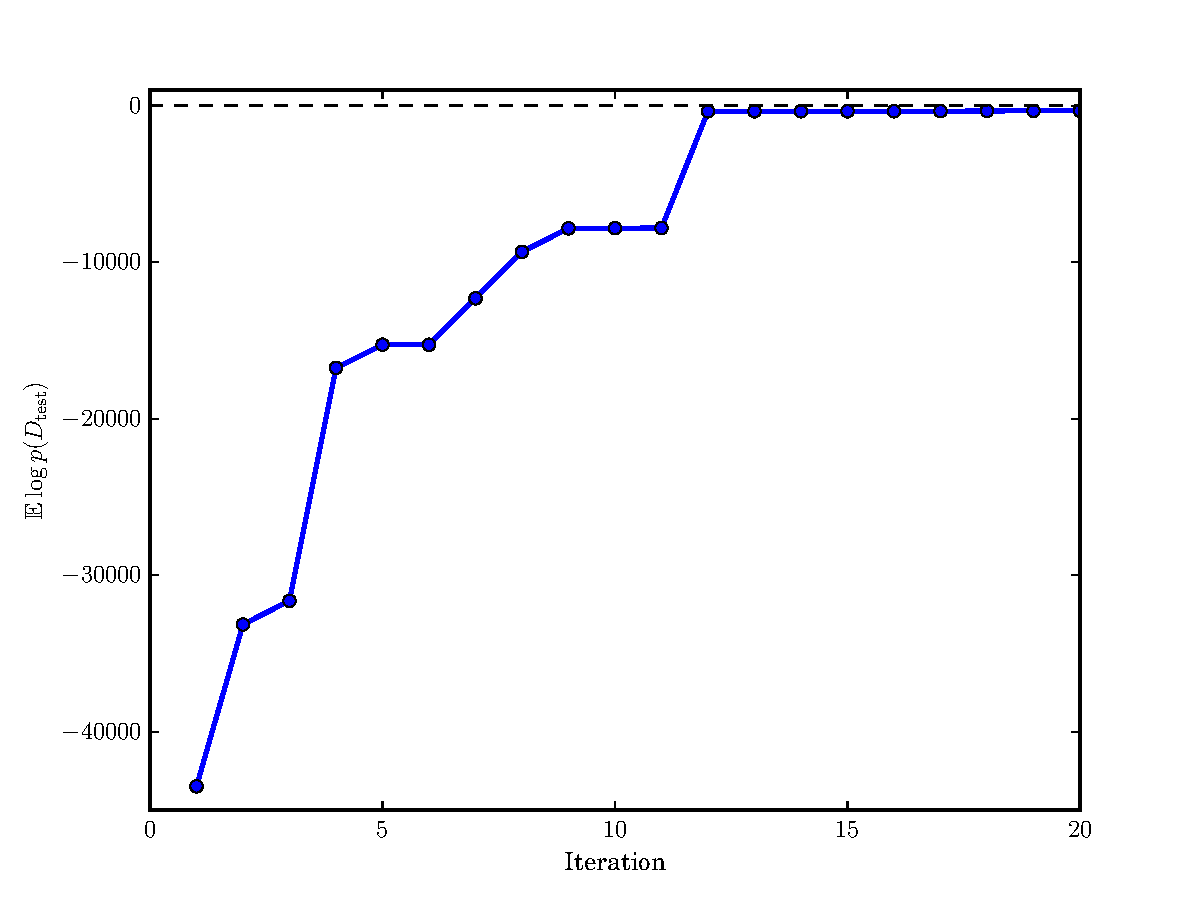
\includegraphics[width=\linewidth]{figures/train_number_net_0006_held_out.pdf}
    \caption{}
    \label{fig:heldoutLL}
  \end{subfigure}
  \caption{(\subref{tab:results}) Viterbi completions of held-out sentences for a 4-predicate 1-layer LPN. (\subref{fig:heldoutLL}) expected log likelihood on a set of held-out test data in a 5-layer LPN with 5 predicates per layer.}
\end{figure}

\section{Preliminary Experiments}

To evaluate LPNs as a probabilistic model of concept acquisition, we
trained a single layer LPN with the architecture in Figure
\ref{fig:architecture} and $K = 4$ latent predicates on a set of
sentences expressing successor and predecessor relations in numbers
between one and ninety-nine. The training set was the collection of
sentences $X = \{\text{after}\, \langle n \rangle \, \text{comes} \,
\langle n+1 \rangle \,|\, n \in 1,\dots,98\} \cup \{\text{before}
\,\langle n \rangle \, \text{comes} \, \langle n-1 \rangle \,|\, n \in
2,\dots,99\},$ where $\langle n \rangle$ is the number words
corresponding to $n$. The lexicon was the set of number word
corresponding to $1$ through $19$, the decades $20, \dots, 90$, the
empty string, and the words ``before'', ``after'', and ``comes''. See
Figure~\ref{fig:parseexample} for a possible LPN derivation of an
example sentence.
%  To approximate the evidence children receive (words
% for small numbers naturally occuring more often than for larger ones,
% but children also rehearse the entire number sequence), we drew these
% sample sentences from a sum of a geometric distribution with parameter
% $0.5$ and a uniform distribution. These components were weighted
% $75\%$ and $25\%$, respectively.
We trained the LPN using $2000$ examples, holding out a subset of
sentences -- including those in Table~\ref{tab:results} -- for evaluation.

% For inference, we used default $\frac{1}{D}$ pseudocounts (where $D$ is the
% dimensionality of the Dirichlet distributions). We found that different random
% initialization for this experiment did not lead to qualitatively different
% results, though further investigation will be necessary to see how
% robust the algorithm is to local maxima when fitting LPNs.

We evaluated the learned model by asking for Viterbi ({\it i.e.}
maximum {\it a posteriori}) completions of the last words of each held
out test sentence. Table~\ref{tab:results} shows some of these
completions. The grammar correctly learns much of the structure of
these sentences, including the difference between sentences starting
with ``before'' and ``after'' and the edge cases that relate decade
words like ``twenty'' to non-decade words like ``twenty one.''

Separately, we trained an LPN with five layers of five predicates each
on a larger dataset including multiple forms of each sentence
(\textit{e.g.} ``twenty comes before twenty one'' and ``before twenty one comes
twenty''). Figure~\ref{fig:heldoutLL} shows the the expected log
likelihood of held out data as a function of algorithm iteration. The
expected log likelihood is a lower bound on the log expected
probability. Its convergence to nearly zero suggests that the trained
LPN discovers the underlying structure of the sentences.

\section{Conclusion}
LPNs allow for tractable learning over a restricted subset of
probabilistic programs. Our preliminary results suggest that LPNs may
enable learning at the intersection of concept learning and language
acquisition, a domain for which an integration of statistical and
symbolic knowledge is particularly promising.



%% Feel free to include if there's space, but this table may not be necessary.
%%
%%   \begin{table}
%%     \centering
%%     \begin{tabular}{>{\tiny} l >{\tiny} l >{\tiny} l >{\tiny} l }
%%       \multicolumn{2}{>{\tiny}l}{$S$(X Y) $\leftarrow$ $A_1$(X, Y) : 1.0000} &      $A_2$(before, comes) : 0.7316 & $A_4$(after, comes) : 0.9990  \\
%%       \multicolumn{2}{>{\tiny}l}{$A_1$(X Y, U V) $\leftarrow$ $A_2$(X, U), $A_3$(V, Y) : 0.5002} & $A_3$(one, two) : 0.3993 & $A_3$(two, three) : 0.2063 \\
%%       \multicolumn{2}{>{\tiny}l}{$A_1$(X Y, U V) $\leftarrow$ $A_3$(Y, V), $A_4$(X, U) : 0.3428} & $A_3$(three, four) : 0.1093 & $A_3$(four, five) : 0.0734 \\
%%       \multicolumn{2}{>{\tiny}l}{$A_1$(X Y, U V) $\leftarrow$ $A_1$(V, Y), $A_4$(X, U) : 0.0796} & $A_3$(five, six) : 0.0502 & $A_3$(six, seven) : 0.0355 \\
%%       \multicolumn{2}{>{\tiny}l}{$A_1$(X Y, U V) $\leftarrow$ $A_1$(Y, V), $A_2$(X, U) : 0.0712} & $A_3$(eight, nine) : 0.0290 & $A_3$(seven, eight) : 0.0271 \\
%%       \multicolumn{2}{>{\tiny}l}{$A_1$(X Y, U V) $\leftarrow$ $A_2$(Y, X), $A_3$(V, U) : 0.0021} & $A_2$(fifty, fifty) : 0.0375 & $A_2$(thirty, thirty) : 0.0361 \\
%%       \multicolumn{2}{>{\tiny}l}{$A_1$(X Y, U V) $\leftarrow$ $A_1$(V, Y), $A_2$(X, U) : 0.0013} & $A_2$(eighty, eighty) : 0.0339 & $A_3$(null, one) : 0.0231 \\
%%       \multicolumn{2}{>{\tiny}l}{$A_1$(X Y, U V) $\leftarrow$ $A_2$(V, X), $A_3$(Y, U) : 0.0008} & $A_2$(forty, forty) : 0.0332 & $A_2$(twenty, twenty) : 0.0310 \\
%%       \multicolumn{2}{>{\tiny}l}{$A_1$(X Y, U V) $\leftarrow$ $A_1$(X, U), $A_2$(V, Y) : 0.0008} & $A_2$(seventy, seventy) : 0.0296 & $A_2$(sixty, sixty) : 0.0274 \\
%%       \multicolumn{2}{>{\tiny}l}{$A_1$(X Y, U V) $\leftarrow$ $A_1$(X, U), $A_2$(Y, V) : 0.0008} & $A_2$(ninety, ninety) : 0.0260 & $A_3$(eighteen, nineteen) : 0.0064 \\
%%       \multicolumn{2}{>{\tiny}l}{$A_1$(X Y, U V) $\leftarrow$ $A_1$(X, U), $A_4$(Y, V) : 0.0004} & $A_3$(sixteen, seventeen) : 0.0049 & $A_3$(eleven, twelve) : 0.0044 \\
%%       $A_3$(nine, ten) : 0.0044 & $A_3$(thirteen, fourteen) : 0.0044 & $A_3$(fourteen, fifteen) : 0.0039 & $A_3$(ten, eleven) : 0.0034 \\
%%       $A_2$(null, fifty) : 0.0043 & $A_3$(eighty, null) : 0.0030 & $A_3$(seventeen, eighteen) : 0.0030 & $A_3$(nine, sixty) : 0.0025 \\
%%       $A_2$(nine, seventy) : 0.0029 & $A_3$(nine, forty) : 0.0020 & $A_2$(null, thirty) : 0.0022 & $A_2$(nine, ninety) : 0.0022 \\
%%       $A_3$(twelve, thirteen) : 0.0015 & $A_3$(fifteen, sixteen) : 0.0015 & $A_3$(null, comes) : 0.0010 & $A_2$(twenty, after) : 0.0014 \\
%%       $A_2$(sixty, before) : 0.0007 & $A_3$(nineteen, comes) : 0.0005 & $A_4$(nine, thirty) : 0.0010 & \\
%%     \end{tabular}
%%     \caption{The 4 predicate LPN trained to model sentences in the number domain. Rules with insignificant weights are removed. This LPN generates the completions in Table \ref{tab:results}.}
%%     \label{tab:grammar}
%%   \end{table}

% To inspect visually the learned grammar, we thresholded rules
% according to the expected number of times they were used in parsing
% the training dataset. Table~\ref{tab:grammar} shows all rules with
% expected count above $1e-6$. This reduces from $2669$ to $52$ the
% number of significant rules. On inspection, predicate $A_2$ forms
% ``before'' sentences, predicate $A_4$ forms ``after'' sentences,
% predicate $A_3$ is successorship recursively defined over the decades
% and ones, and predicate $A_2$ is a category for the decade words.

% Our LPN does not learn to how to transition between the last word in a decade
% and the next decade (e.g. ``seventy nine'' to ``eighty''). Instead, it
% makes the intuitively reasonable generalization that ``seventy nine''
% should be followed by ``seventy ten.''


\bibliographystyle{plain}
\bibliography{nips_workshop}

% \nocite{*}

\end{document}
